\documentclass{article}
\usepackage{listings}
\usepackage{graphicx}
\usepackage{color}

\definecolor{mygreen}{rgb}{0,0.6,0}
\definecolor{mygray}{rgb}{0.5,0.5,0.5}
\definecolor{mymauve}{rgb}{0.58,0,0.82}

\lstset{ %
  backgroundcolor=\color{white},   % choose the background color; you must add \usepackage{color} or \usepackage{xcolor}; should come as last argument
  basicstyle=\footnotesize,        % the size of the fonts that are used for the code
  breakatwhitespace=false,         % sets if automatic breaks should only happen at whitespace
  breaklines=true,                 % sets automatic line breaking
  captionpos=b,                    % sets the caption-position to bottom
  commentstyle=\color{mygreen},    % comment style
  deletekeywords={...},            % if you want to delete keywords from the given language
  escapeinside={\%*}{*)},          % if you want to add LaTeX within your code
  extendedchars=true,              % lets you use non-ASCII characters; for 8-bits encodings only, does not work with UTF-8
  frame=single,	                   % adds a frame around the code
  keepspaces=true,                 % keeps spaces in text, useful for keeping indentation of code (possibly needs columns=flexible)
  keywordstyle=\color{blue},       % keyword style
  language=Octave,                 % the language of the code
  morekeywords={*,...},           % if you want to add more keywords to the set
  numbers=left,                    % where to put the line-numbers; possible values are (none, left, right)
  numbersep=5pt,                   % how far the line-numbers are from the code
  numberstyle=\tiny\color{mygray}, % the style that is used for the line-numbers
  rulecolor=\color{black},         % if not set, the frame-color may be changed on line-breaks within not-black text (e.g. comments (green here))
  showspaces=false,                % show spaces everywhere adding particular underscores; it overrides 'showstringspaces'
  showstringspaces=false,          % underline spaces within strings only
  showtabs=false,                  % show tabs within strings adding particular underscores
  stepnumber=2,                    % the step between two line-numbers. If it's 1, each line will be numbered
  stringstyle=\color{mymauve},     % string literal style
  tabsize=2,	                   % sets default tabsize to 2 spaces
  title=\lstname                   % show the filename of files included with \lstinputlisting; also try caption instead of title
}

\author{Jacob Hutter}
\title{ECE 311 Lab 3}

\begin{document}
\maketitle

\begin{figure}[H]
\ Report Item 1
\lstinputlisting[language=Matlab]{myDFTConv.m}
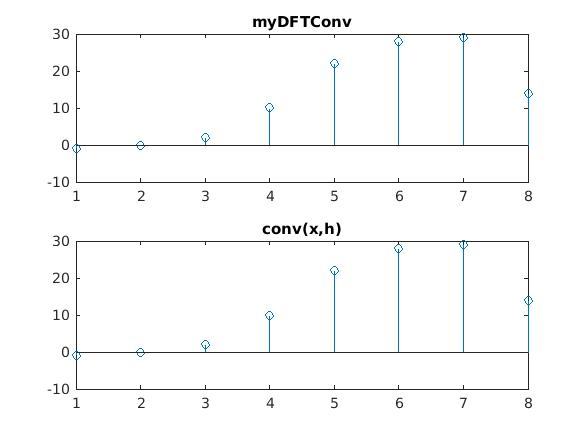
\includegraphics[scale = .5]{report1}
\\ Because of the use of fft and ifft, the time coplexity is also $O(Nlog(N))$.
\end{figure}



\begin{figure}[H]
\ Report Item 2
\lstinputlisting[language=Matlab]{sys1.m}
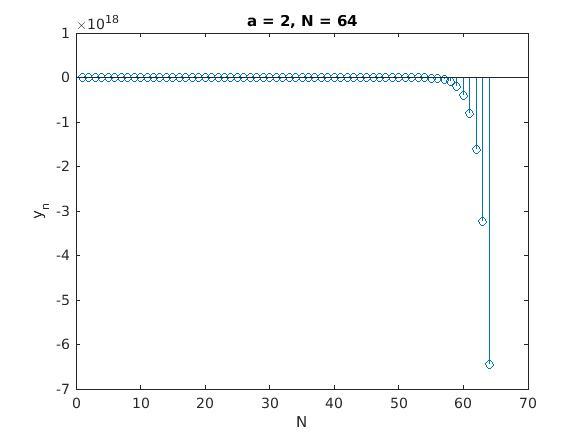
\includegraphics[scale = .5]{report2}
\\ Notice that this function is in the order of a negative exponential, 
therefore, it is not stable $\lim_{N\to\infty} y_n = -\infty$.
The system is causal, however, by the finite difference equation, output only 
depends on past or current inputs.
\end{figure}

\begin{figure}[H]
\ Report Item 3
\lstinputlisting[language=Matlab]{sys2.m}
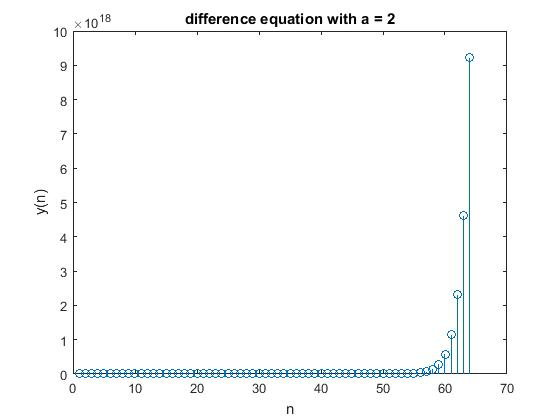
\includegraphics[scale = .5]{report3}
\\ With $a = 2$ and $x(n) = (1,0,0,....)$, or the delta function, we can see that the equation is not linear because of $x(n)^{2}$. The system is causal because of the fact that the finite difference equation output only depends on past or current inputs. Because the output graph is in the form of an exponential, the equation is unnstable.
\end{figure}
\begin{figure}[H]
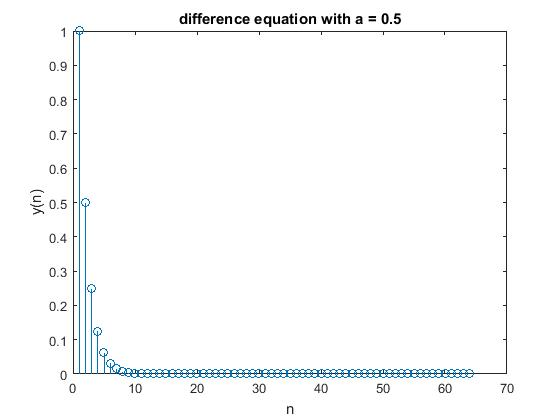
\includegraphics[scale = .5]{report3_2}
\\ With $a = 0.5$, the equation is not linear, causal, and is stable because $\lim_{N\to\infty} y_n = 0$.
\\ Because the equation is not linear, the system is not LSI so you cannot use convolution to find the output to either system.
\end{figure}

\begin{figure}[H]
\ Report Item 4
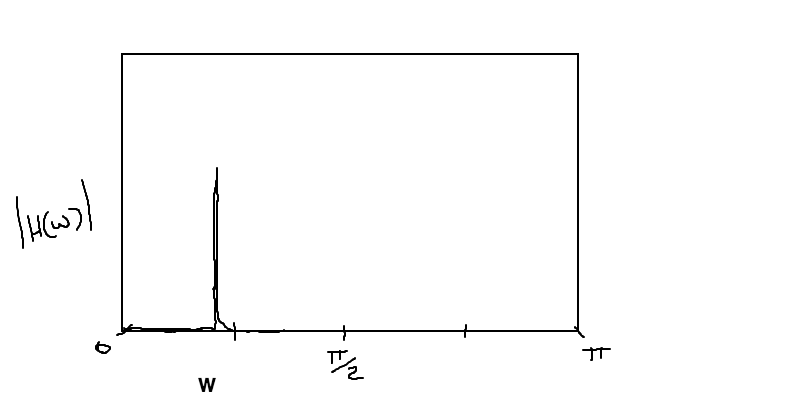
\includegraphics[scale = .5]{report4_1}
\ We can see on the interval from $\omega$ = $0$ to $\pi$, that there is only one point where the magnitude is not zero. Therefore, there is a spike at that point.
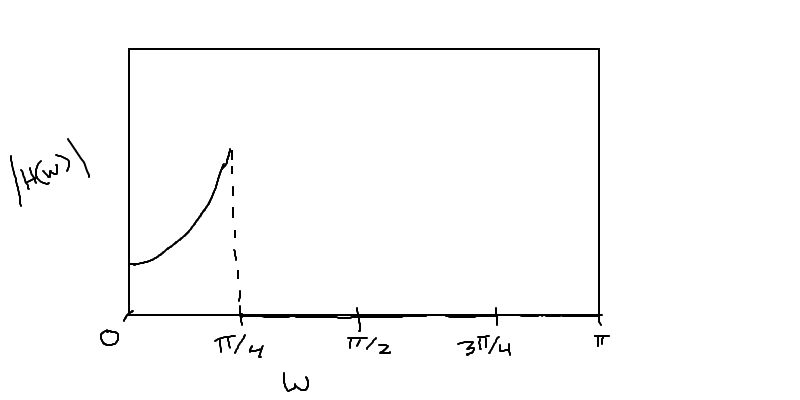
\includegraphics[scale = .5]{report4_2}
\ We can see on the interval from $\omega = 0$ to $\pi $ that there is a minimum at $\omega = 0$ and a maximum at ~ $\omega = \pi/4$ so the graph is decreasing until that point.
\end{figure}

\begin{figure}[H]
\ Report Item 5
\lstinputlisting[language=Matlab]{pzplot_impz.m}
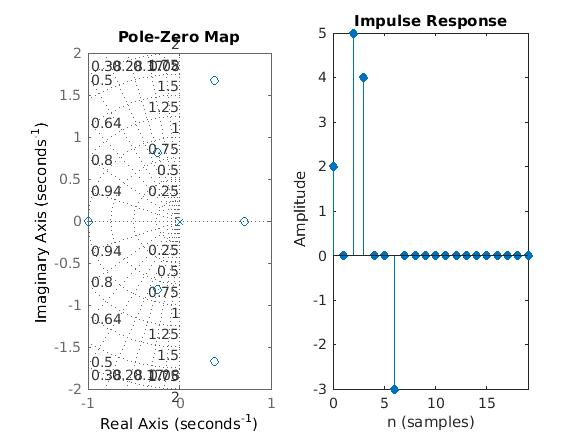
\includegraphics[scale = .5]{report5_1}
\\ With $a = [1,0,0,0,0,0,0]$ and $b =[2,0,5,4,0,0,-3]$
\ There are no poles on or outside the unit circle so the system is stable.
\end{figure}

\begin{figure}[H]
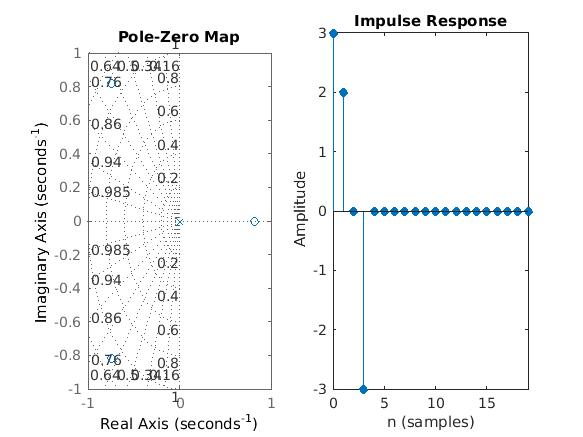
\includegraphics[scale = .5]{report5_2}
\\ With $a = [1,0,0,0]$ and $b = [3,2,0,-3]$, there are no poles on or outside the unit circle. Therefore, the system is stable.
\end{figure}

\begin{figure}[H]
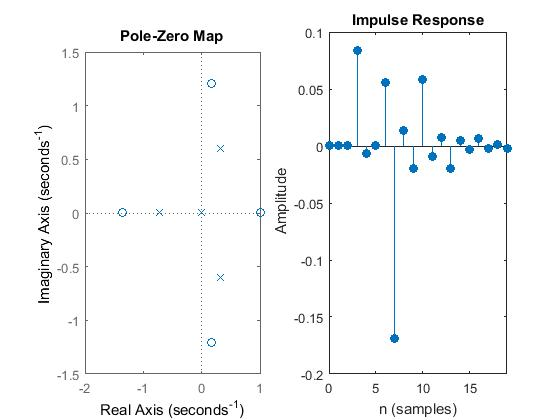
\includegraphics[scale = .5]{report5_3}
\\ With $a = [12,1,0,4,0,0,0,0]$ and $b =[0,0,0,1,0,0,1,-2]$, there are no poles outside or on the unit circle. Therefore, the system is stable.
\end{figure}

\begin{figure}[H]
\ Report Item 6
\\ $H(z) = \frac{z}{{(z+e^{\frac{-i8\pi}{10}})(z+e^{\frac{i8\pi}{10}})}}$
\\ $ = \frac{z}{z^2 + ze^{\frac{-i8\pi}{10}} + ze^{\frac{i8\pi}{10}} + 1}$
\\ $ = \frac{z}{z^2+2zcos(4\pi/5) + 1}$
\\ $ = \frac{z^{-1}}{1 + z^{-1}2cos(4\pi/5) + z^{-2}}$
\\ $ a = [1,2cos(4\pi/5),1], b = [0,1,0]$
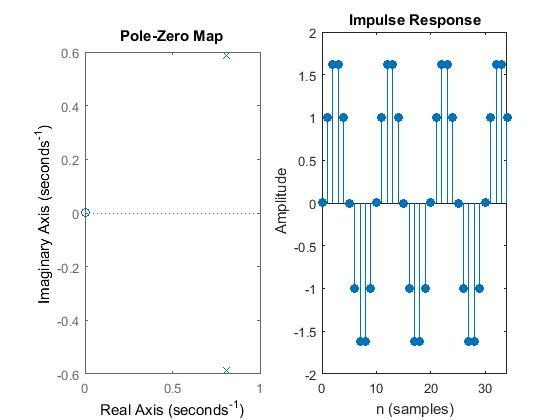
\includegraphics[scale = .5]{report6}
\\ The system is not BIBO stable, we have two poles on the unit circle.  The system is stable when $|z| < e^{\frac{\pm i8\pi}{10}}$ and unstable when $|z| =  - e^{\frac{\pm i8\pi}{10}}$.
\end{figure}



\break

\end{document}
